\chapter{Datasets Construction}
\label{datasets_construction}
One of the main challenges of this project is the construction of datasets capable of representing as faithfully as possible the reality of tables in newspapers. This chapter first focuses on the definition of tables in \ref{on_the_definition_of_tables} to make the reader aware of the difficulty of defining this layout element. It then explains where the data used in this project comes from in \ref{data_sources}. Subsequently, in \ref{annotation_processes}, it delves into the data itself by commenting on its annotations, deriving meaningful statistics and visualizations, and expanding on the creation of the datasets used in the experiments. Finally, a summary of the datasets constructed for the experiments is given in \ref{datasets_summary}.

\section{On the definition of tables}
\label{on_the_definition_of_tables}
This section is meant to serve as an entry point to the layout object that is a table, and in particular through the prism of newspapers. Defining what are tables or tabular data is actually not a trivial decision. Indeed, most of the popular definitions of table only describe them as a list or an arrangement of data in a system of rows and columns. There is no obvious formal definition and therefore a lot of room is left for interpretation. How many rows and how many columns does a table need to be considered as such, does the title or header of a table is part of the said table, do rows and/or columns delimiters need to be visually present, do they need to be aligned? Many questions arise when one is asked to define a table and many more follow when asked to annotate tables in newspapers. \\

Figure \ref{panel_tables} gathers examples of tables encountered during the realisation of this project and illustrate their diversity, with complete, ``classical'' tables (e.g. (d) or (j)), some having complex arrangements (h), and others resembling more to lists (b). In a document that provides guidelines for annotating tables in newspapers -- to which we will return later --, the National Library of Luxembourg defines tables as ``data structures composed of a series of data of the same type and have a tabular layout where the number of columns is fixed from the start. Tables can have a title and they are used inside section or articles.''. In a survey on table recognition, \cite{zanibbi_survey_2004} say tables serve to ``visualize indexing schemes for relations'' where ``the sets of a relation underlying a table are called domains or dimensions. A relation may be presented in many different ways in a table. Dimensions may be laid out in different row and column arrangements, repeated, or ordered in various ways. The arrangement of dimensions in a table affects which data are most easily accessed and compared.''.  \\

The presence of columns seem to be one of the most important characteristics a table must fulfill to be considered as such. It also seems to be important to have data that makes sense together. Examples like (f) may also raise questions too, even though most people would agree that it is not a table, a row and column arrangement can be guessed at in some way, with the number of columns changing between rows. (b) could be seen as a table with one row and several columns, which is spread on multiple lines because of the layout constraint of the medium. It is easy to find ways to fit the description of tables to any ambiguous cases. In fact, it seems that a formal definition is too difficult to achieve, as any arrangement of data could be considered a table. As we will see later, it is probably better to settle on a more restrictive definition, e.g., by setting a minimum number of columns and rows or by requiring specific visual delimiters, which corresponds to the tasks at hand. It seems complicated, for example, to expect a visual model to understand that say examples (f) and (n) are both tables, since their visual features largely differ.

\begin{figure}
\centering
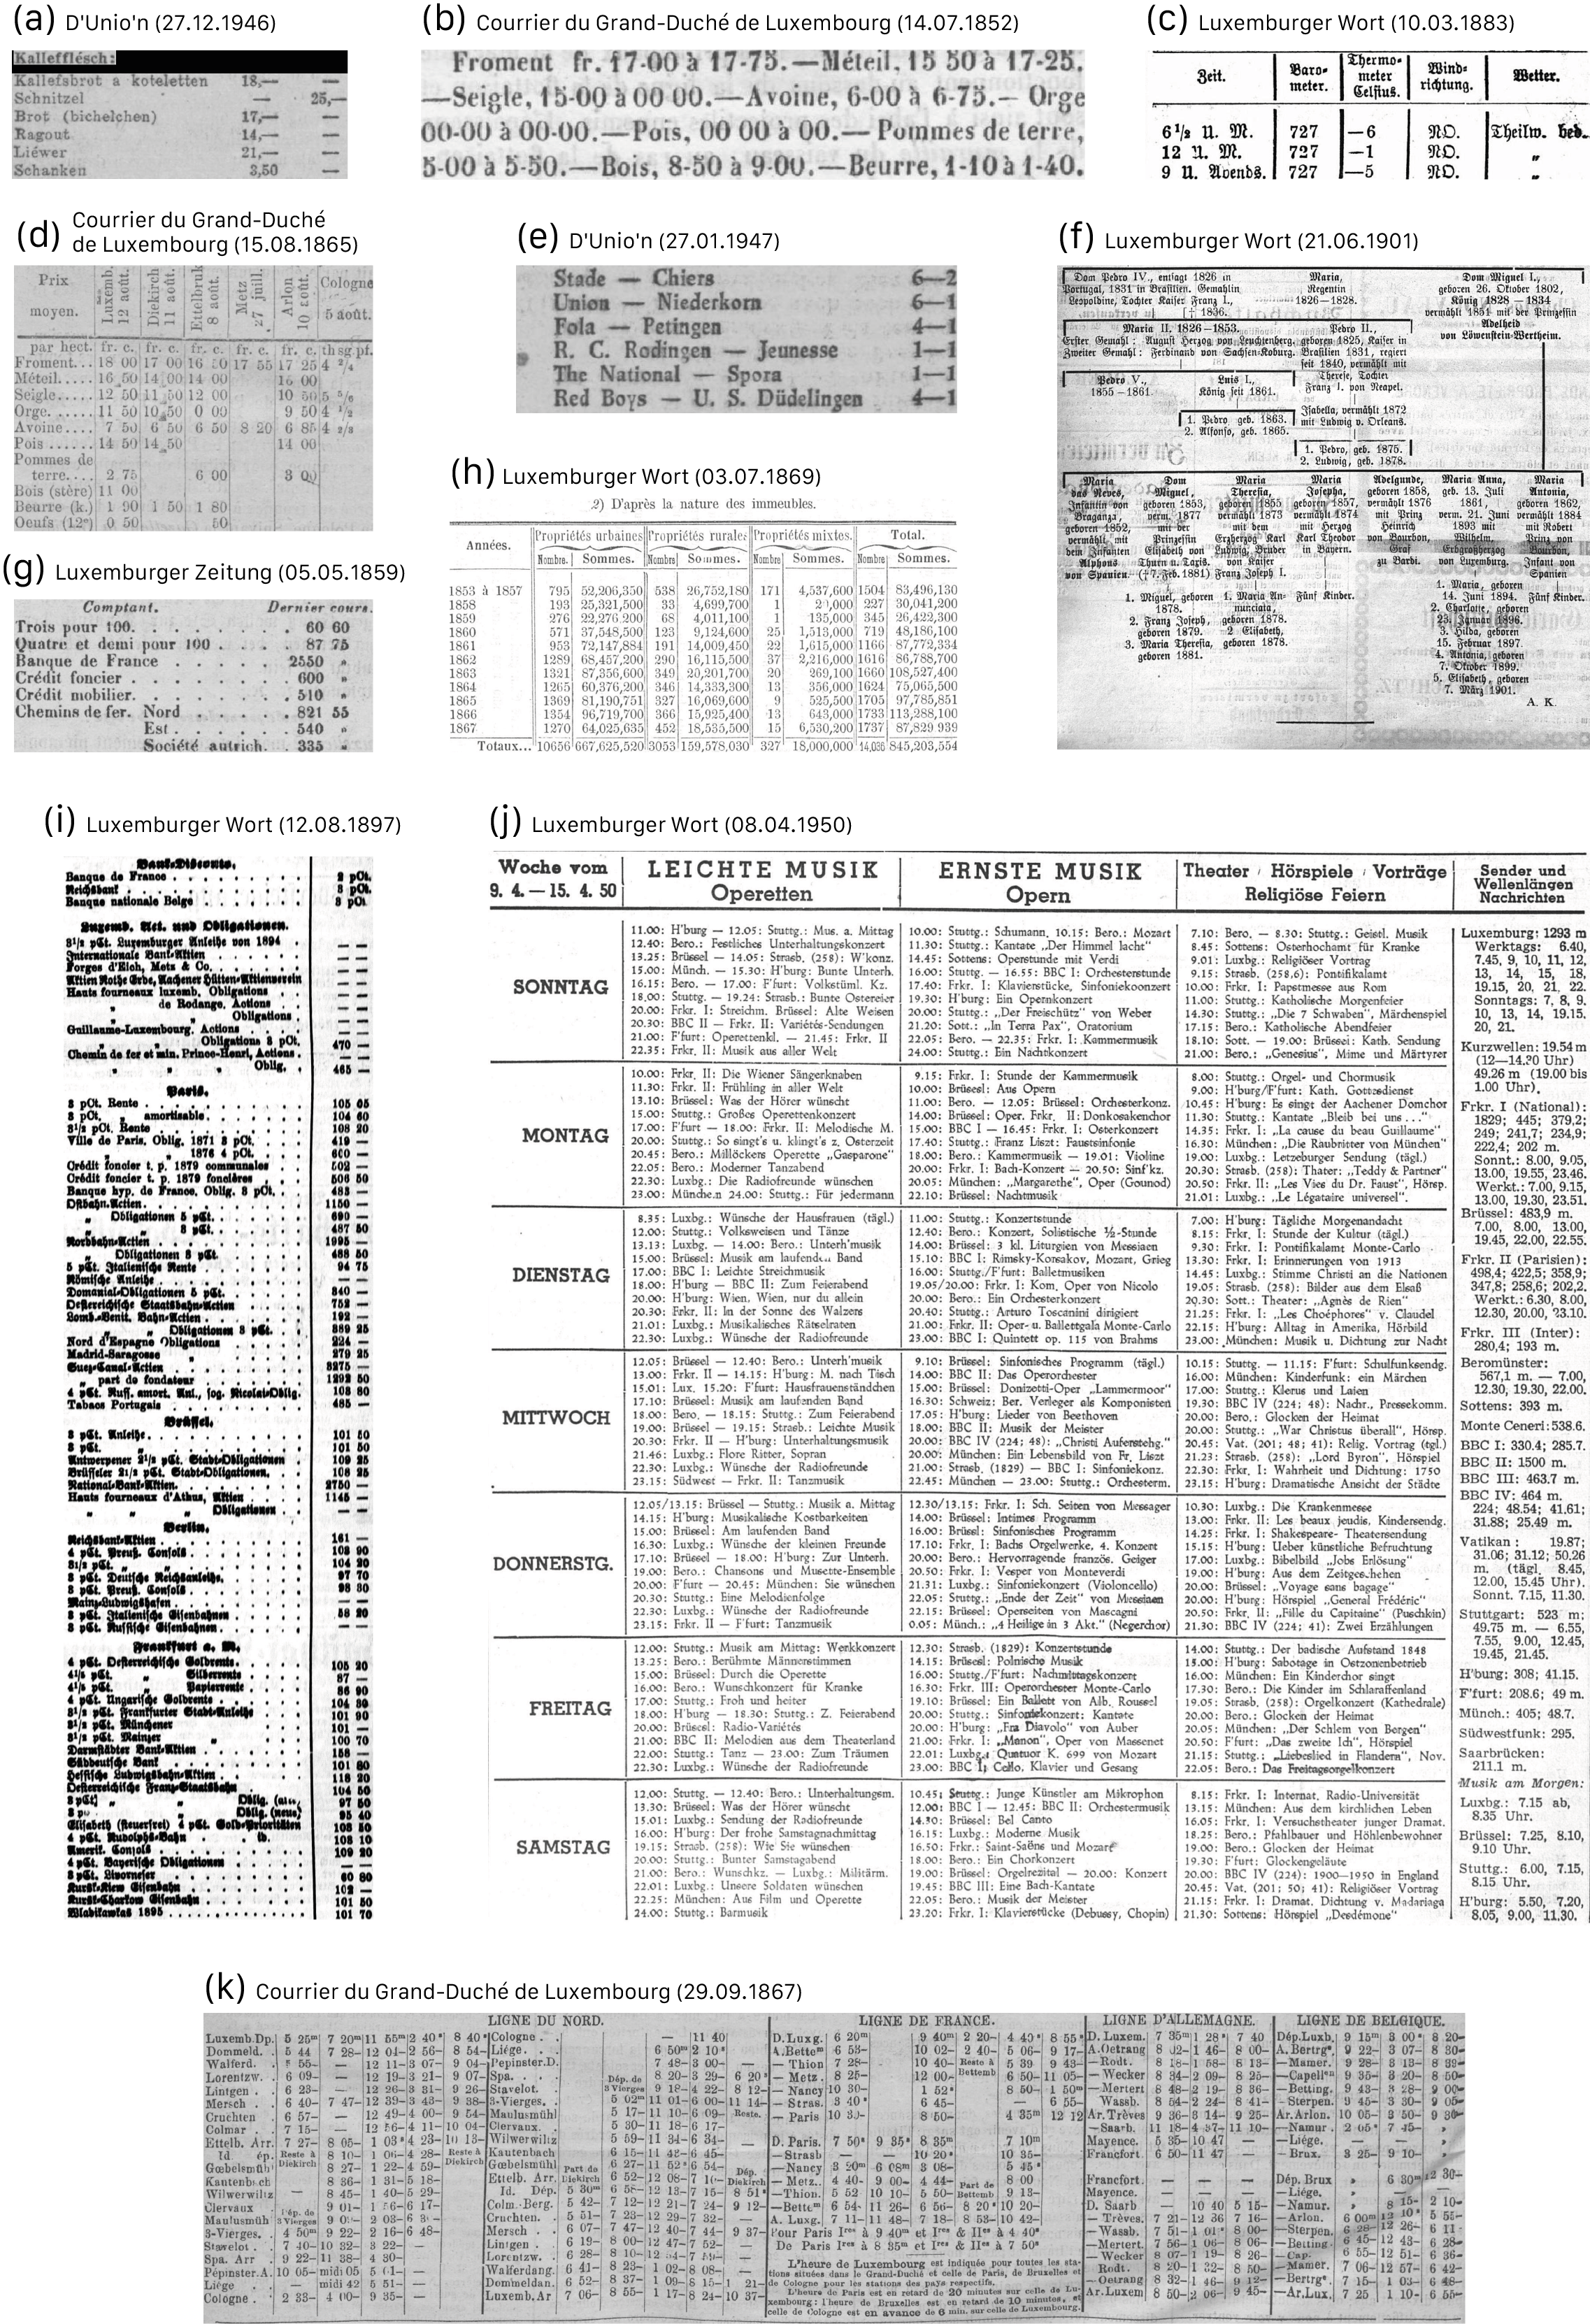
\includegraphics[width=0.95\textwidth]{panel_tables.jpg}
\caption{A panel of tables encountered during the development of the project.}
\label{panel_tables}
\end{figure}

\section{Data sources}
\label{data_sources}
Two different sources were explored to build datasets for table detection and table classification. 

\subsection{Newspaper dataset of the National Library of Luxembourg}
The National Library of Luxembourg, a partner in the \textit{impresso} project, has granted access to its scanned collection of newspapers, which has the particularity of containing segmented portions of the newspaper pages annotated as tables. The data consists of high-resolution scans of Luxembourgish newspapers pages accompanied by rectangular pixel coordinates delineating the locations of the different layout elements on these scans. Segmentation was obtained by applying Optical Layout Recognition (OLR) methods. In addition, an Optical Character Recognition (OCR) was performed and the output is accessible as text tokens with their associated bounding box coordinates. \\
Originally, the dataset was constructed semi-automatically, i.e., tables were detected automatically and then a sample was checked manually. If the number of errors in the sample was within established limits, the overall segmentation was considered correct. Some details on this process are given on a document setting the technical requirements available online.\footnote{\url{https://data.bnl.lu/data/historical-newspapers/}} In summary, five out of every thousand issues were sampled and the maximum number of errors (categorized as blocking, minor or major errors) allowed was set across all types of newspaper items combined. No blocking errors were tolerated, and a maximum of one major and four minor errors were allowed per sixteen pages in a single issue. An exhaustive list of what is considered an error is given in the technical requirements of the library. Unfortunately, this means that it is not possible to draw any solid conclusions about the quality of table annotations of tables in particular. Nevertheless, because of the high standards set by the library, this data provided a seemingly perfect starting point for creating a representative dataset of newspaper tables.\\
As mentioned, OLR was applied to all newspaper pages to identify their constituent elements. These elements are often associated with an instance of a larger layout object. Figure \ref{nll_segmentation_articles} gives an idea of the original segmentation provided by OLR where each color corresponds to one of these instances. For simplicity, we will henceforth refer to these instances as articles or journal items. As can be seen, several bounding boxes can be associated with a single article. Note also that some parts of the page (e.g. the masthead) have not been segmented. Figure \ref{nll_segmentation_tables} shows only the segmentation of articles labelled as table. Note how an instance of a table can also be split in multiple bounding boxes. This is because the titles as well as the sources of the data used in the table (as in the Figure) are often segmented separately from the table itself. The overall segmentation should therefore be taken with a grain of salt, as it may not exactly represent the original segmentation made by the journal editors.

\begin{figure}
\centering
\begin{tabular}{cc}
\subfloat[All types of articles (from Luxemburger Zeitung (10.03.1858), page 1)\label{nll_segmentation_articles}]{\includegraphics[width=0.45\textwidth]{nll_segmentation_articles.png}} &
\subfloat[Tables only (from d'Letzeburger Land (15.05.1987), page 14)\label{nll_segmentation_tables}]{\includegraphics[width=0.45\textwidth]{nll_segmentation_tables.png}}
\end{tabular}
\caption{Original segmentation of newspaper pages coming from the collection of the National Library of Luxembourg.}
\end{figure}

\subsubsection{Statistical exploration}
\label{nll_exploration}
The dataset of the National Library of Luxembourg consists of 58,011 articles labelled as tables distributed across 28,497 pages, themselves spread over 22,735 different newspaper issues. Figure \ref{issue_distribution} shows the distribution of these 22,375 issues with annotated tables over time, relative to the full \textit{impresso} Luxembourg newspaper corpus, which contains 65,515 different issues. This highlights the skewed temporal distribution of the table dataset, where issues appearing before circa 1875 are over-represented. This could generate some bias towards tables that appear only during this period. A similar distribution is observed when comparing the distribution over time of the pages of the table dataset vs. of the full Luxembourg \textit{impresso} corpus (352,137 pages) (Figure \ref{page_distribution}), and the distribution of tables vs. of the 2,372,990 articles (Figure \ref{article_distribution}). It is difficult to draw a conclusion as to whether or not the use of tables in newspapers was more prominent towards the years 1855-1875. However, under the assumption that the number of newspaper issues containing at least one table is stable over the years, Figure \ref{issue_distribution} might indicate that the automatic detection of tables by OLR did not perform equivalently across issues and/or time.  \\

\begin{figure}
\centering
\begin{tabular}{c}
\subfloat[Distribution of the issues\label{issue_distribution}]{\includegraphics[width=0.67\textwidth]{issue_distribution.png}} \\
\subfloat[Distribution of the pages\label{page_distribution}]{\includegraphics[width=0.67\textwidth]{page_distribution.png}} \\
\subfloat[Distribution of the articles\label{article_distribution}]{\includegraphics[width=0.67\textwidth]{article_distribution.png}}\\
\subfloat[Distribution of the average size of tables\label{table_size_normalized}]{\includegraphics[width=0.67\textwidth]{table_size_normalized.png}} \\
\end{tabular}
\caption{Distributions over the years for the data of the National Library of Luxembourg.}
\end{figure}

In order to get additional insights on the legacy OLR from the National Library of Luxembourg for the case of tables, Figure \ref{table_size_normalized} shows the mean and standard deviation of the pixel area (normalized by the page area) tables take in pages that contain at least one table. We see that the average area occupied by tables in pages appears to increase slightly over time. Many interpretations are possible at this point. It could be due to a change in the layout of newspapers, which evolved from very condensed (possibly due to printing costs) to more spaced out through time. It could also point towards inconsistent annotation: assuming that the number of tables is constant over time, it is possible that tables in the later years actually contain multiple tables, thus increasing their average area and diminishing their numbers (as seen in Figure \ref{article_distribution}).\\
Finally, Figure \ref{pages_per_journal} shows the number of pages per title that contain tables, while Figure \ref{pages_per_journal_normalized} compares these values to the total number of pages per journal. Some titles, such as the \textit{Luxemburger Wort} (luxwort), have a lot of pages with tables (24,159) but these pages amount only to a small percentage (2.18\%) of their total pages, while other titles, such as the \textit{Luxemburger Zeitung} (luxzeit1858), are in the opposite situation, i.e., they have a large percentage of their pages that contain tables (13.14\%) but these only amount to a low total number (1,623). This discrepancy in percentages could be explained by the types of articles (perhaps more data-oriented) or the layout of the journal, which makes it easier during OLR to detect the tables.

\begin{figure}
\centering
\begin{tabular}{cc}
\subfloat[Pages with tables\label{pages_per_journal}]{\includegraphics[width=0.45\textwidth]{pages_per_journal.png}} &
\subfloat[Ratio of pages with tables normalized over total number of pages\label{pages_per_journal_normalized}]{\includegraphics[width=0.45\textwidth]{pages_per_journal_normalized.png}}\\
\end{tabular}
\caption{Distributions of the number of pages for each journal.}
\end{figure}

\paragraph{Dataset naming}
In order to facilitate writing and overall understanding, the dataset consisting of all the pages that make up the National Library of Luxembourg collection will now be referred to as \textbf{NLL-full}. The subset of \textbf{NLL-full} consisting solely of pages containing articles labelled as tables will be referred to as \textbf{NLL}.

\subsection{Raphaël Barman's Master project}
\citet{barman_historical_2019} is a Master project previously conducted at the EPFL-DHLAB that explored the ability of a visual model integrating textual clues to segment certain classes of articles in newspapers archives. During this project, a dataset had to be built with manually annotated and tagged articles. The tag set used included \textit{stock exchange tables} that fit exactly what we were looking for. This dataset seemed to be an excellent way to quickly increase the amount of relevant data, while also providing some diversity. Indeed, the dataset was constructed by sampling only from Swiss-French newspapers, which should differ in some way from Luxembourgish newspapers in terms of layout and language. The sampling was done on three journals, the \textit{Journal de Genève} (JDG), \textit{L'Impartial} (IMP) and the \textit{Gazette de Lausanne} (GDL), by randomly taking three issues every 3 or 5 years depending on the journal. Figures \ref{rb_segmentation_tables} and \ref{rb_segmentation_tables2} show some examples from this dataset. The tables have been annotated at the pixel level, which means that an instance of a table can contain multiple tables. Finally, it should be noted that due to the smallness of the dataset, it was quick to verify whether every annotated stock exchange tables were indeed tables: surprisingly, 24 had to be removed. We should point out that it is possible that some tables, which were not stock exchange tables, were not annotated, making this dataset slightly inconsistent. 

\begin{figure}
\centering
\begin{tabular}{cc}
\subfloat[Gazette de Lausanne (15.02.1997), page 19\label{rb_segmentation_tables}]{\includegraphics[width=0.45\textwidth]{rb_segmentation_tables.png}} &
\subfloat[Journal de Genève (23.02.1867), page 3\label{rb_segmentation_tables2}]{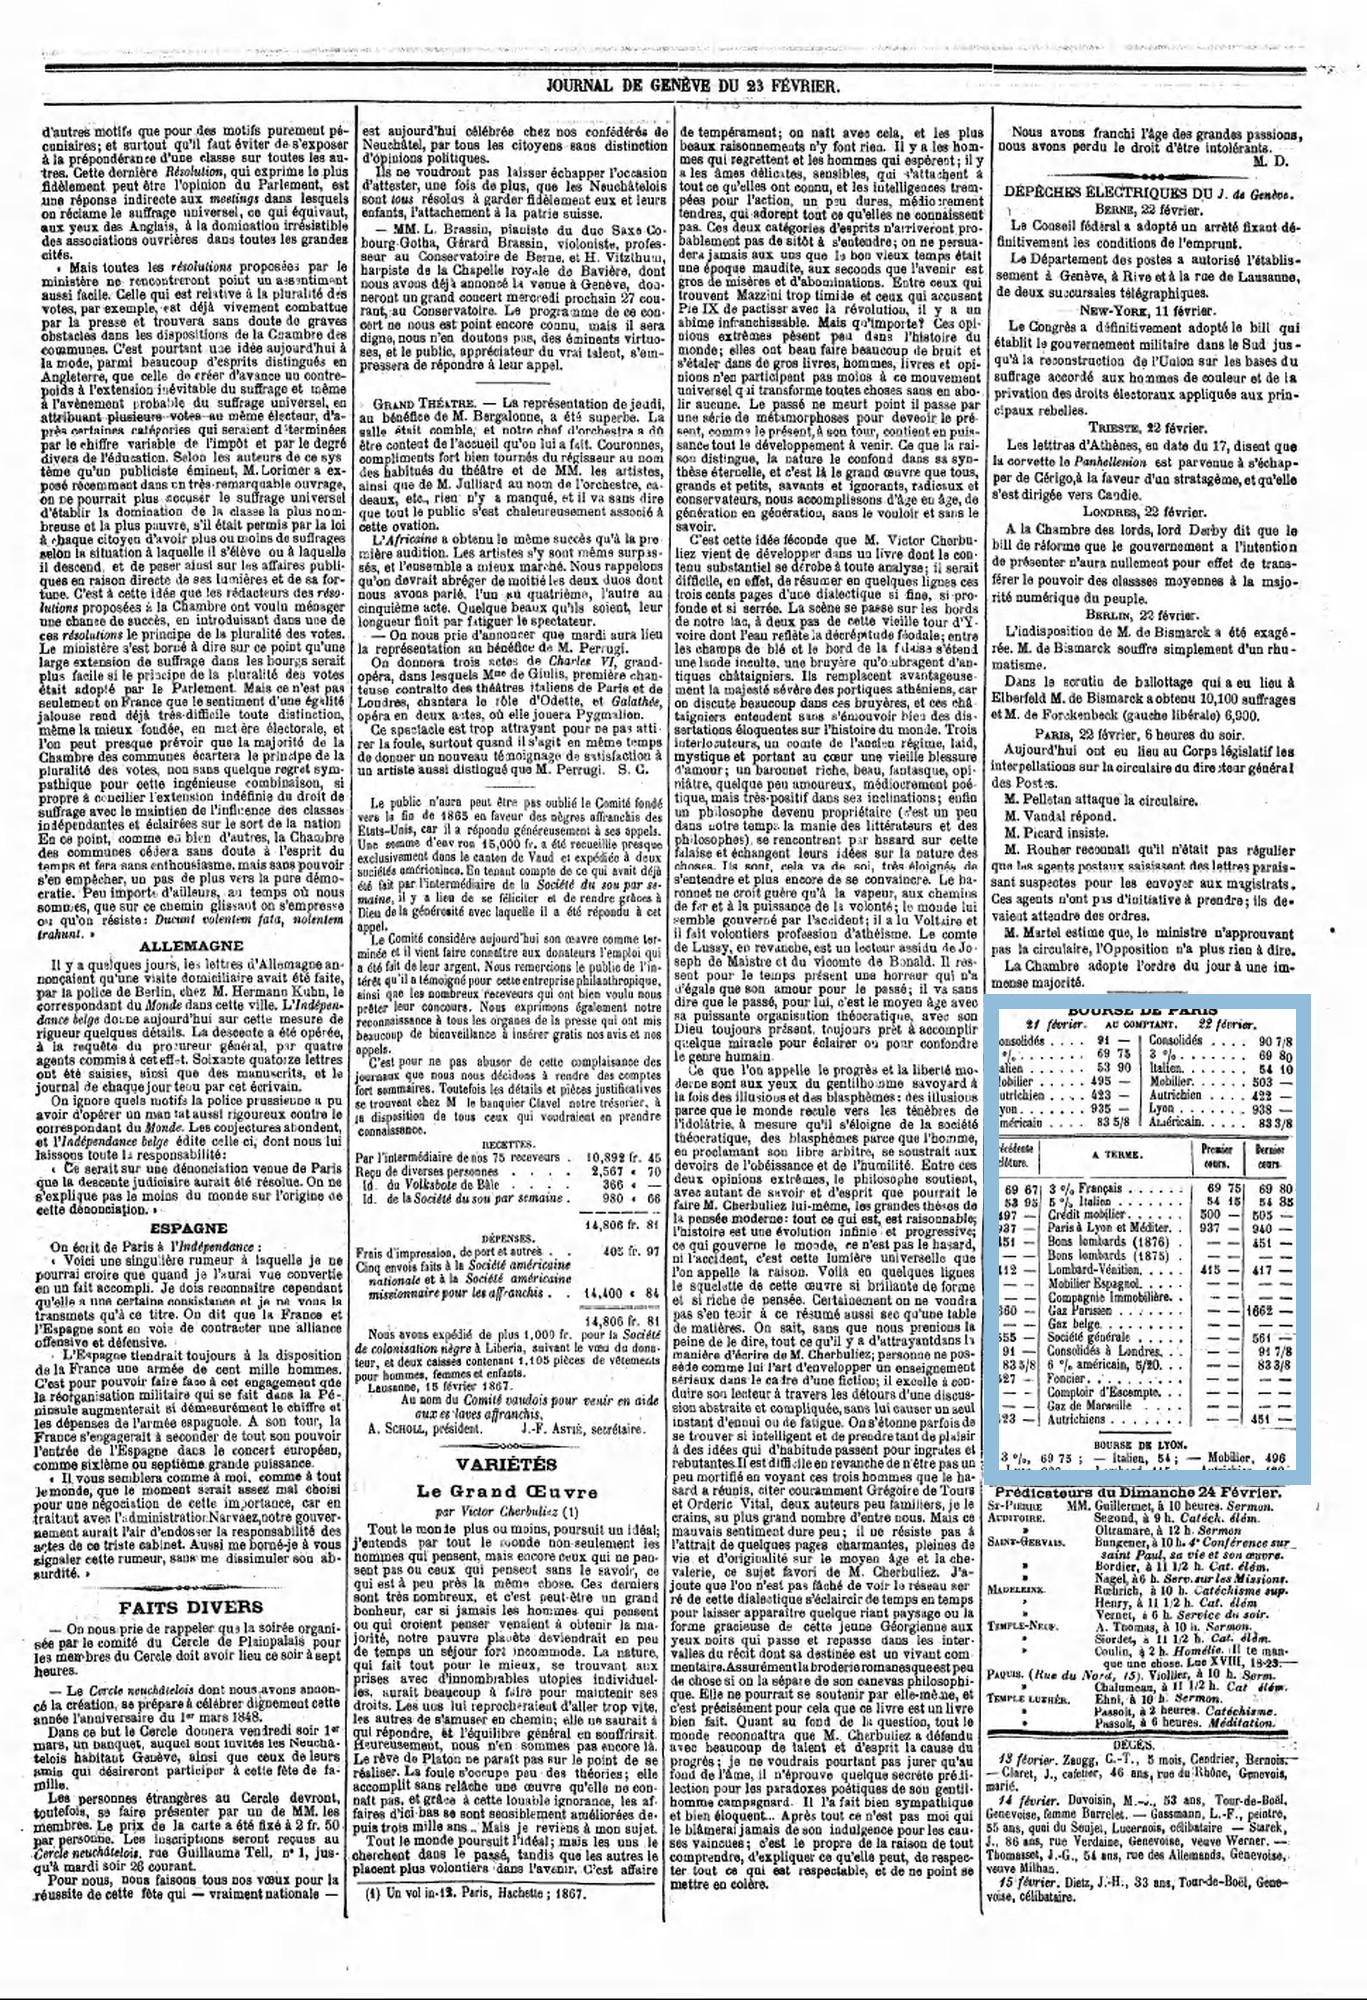
\includegraphics[width=0.45\textwidth]{rb_segmentation_tables2.png}}\\
\end{tabular}
\caption{Original segmentations of newspaper pages coming from \citet{barman_historical_2019}.}
\end{figure}

\subsubsection{Statistical exploration}
In total, the dataset contains 800 tables spread over 474 pages from 3 different titles, themselves spread over 311 issues. Figure \ref{rb_page_distribution} shows the distribution of pages over time for each title. JDG is the most prominent journal because it was sampled every 3 years while the other two were sampled every 5 years. We can notice that stock exchange tables seem to be more numerous between circa 1985 to 1995, with a drop between circa 1915 and 1975.

\begin{figure}[h]
\centering
\includegraphics[width=0.75\textwidth]{rb_page_distribution}
\caption{Distribution over time of the number of pages containing stock exchange tables coming from \citet{barman_historical_2019}.}
\label{rb_page_distribution}
\end{figure}

\paragraph{Dataset naming}
From now on, the dataset containing these 474 pages with stock tables will be referred to as \textbf{RB}.

%\subsection{ICDAR}
%The International Conference on Document Analysis and Recognition (ICDAR) is an academic conference held every two years which proposes competition on different topic centred around %document analysis. In 2019, a competition on Table Detection and Recognition (cTDaR) \cite{gao_icdar_2019} took place in which a large dataset consisting of documents containing all %sorts of tables: printed, handwritten, historical, modern. This dataset was investigated in order to assess the interest in providing out-of-domain examples to the models.

%\paragraph{Dataset naming}
%This dataset will be referred to as \textbf{cTDaR}.

%\section{Data retrieval and infrastructure}
%\label{data_retrieval_and_infrastructure}
%TODO explain the technical challenges  SOLR IFFF S3

\section{Annotation processes}
\label{annotation_processes}
The many annotation processes of \textbf{NLL} undertaken are detailed here in the order they were conducted. Initially, a subset had to be classified in order to tackle the task of table classification. After this initial annotation, a process to increase the size of the already labelled dataset by automatically tagging tables based on the previous manual annotation was explored. After some initial experiments, problems within \textbf{NLL} were revealed and needed to be investigated. The creation of a dataset that attempts to attenuate them based on a statistical exploration is explained, as well as the motivations behind the creation of a final dataset with properly annotated ground truth.

\subsection{Manual classification of tables}
\label{manual_classification_of_tables}
Since one of the goal of the project was to classify tables under finer grained semantic classes, it was decided to dig deeper into \textbf{NLL} through a manual pass in order to tag some tables and identify a typology that could cover all types of tables found in newspapers across time.

\subsubsection{Annotation tool}
In order to alleviate the traditional pains that accompany any annotation process, a web application was developed as a support tool to efficiently browse datasets consistent with this project's case study, i.e., images (tables in this case) cropped out from larger images (newspaper pages in this case). The tool allows the user to increase their tagset as they go through the dataset and discovers new classes. In Figure \ref{letagger}, the application interface can be seen. The left-hand side displays the complete list of tables that can be browsed by category (tagged/untagged/tagged by class), while on the right-hand side are displayed the images similar to the image on the left.\\
Sometimes the legacy segmentations of \textbf{NLL} poorly frame the tables to be tagged; the annotator will then need additional contextual clues to correctly classify the table. In such cases, it becomes necessary to zoom out and look at the entire newspaper page, which is easily achievable with this tool, thus ensuring a qualitative annotation process. In addition, the tool also allows the user to quickly query images that resemble the one they are looking at, provided the dataset meets the infrastructural requirements. This aspect of the tool is discussed in more detail in \ref{automatic_classification_of_tables}.\\

\begin{figure}[h]
\centering
\includegraphics[width=0.9\textwidth]{letagger.png}
\caption{A view of the web application developed to support the annotation processes undertaken during the project.}
\label{letagger}
\end{figure}

\subsubsection{Annotation process}
Using the annotation tool, we needed to create a typology robust enough that it could efficiently summarize \textbf{NLL}. A total of 3,787 tables were manually classified, which amounts to 6.53\% of the tables in \textbf{NLL}. The annotation was done in three different phases. In the first phase, 525 tables were sampled completely at random. We noticed a lack of visual dissimilarity between tables, likely due the skewed temporal distribution (a characteristic problem of \textbf{NLL} raised before), which motivated a revision of the annotation process. Indeed, since most of the sampled tables came from the over-represented periods, many of them were extremely similar, if not identical, tables. Newspapers often use the same tables across multiple issues for recurring topics, such as transport schedules or stock exchanges. Another reason for the decision to revise the process was the need for a robust typology over several years. Indeed, one could hardly come up with a class for radio or television programs if only tables prior to 1900 are sampled. To overcome this problem, and thus better capture the diachronic properties of the domain under study, both visually and semantically, 491 tables were sampled according to the year they originate from, with a probability inversely proportional to the number of tables coming from that year in the dataset. In short, each year had the same probability of being drawn.\\

\paragraph{Established typology}
Through this annotation process, 12 classes were identified. For each of them an example from Figure \ref{panel_tables} is given as well as the number of items classified:
\begin{itemize}
\setlength\itemsep{0em}
\item transport schedule: train and bus timetables (2,301 items, see example (o));
\item sport results: tables that contain sport results, or sport rankings (403 items, see example (e));
\item stock: tables that contain data related to the stock markets (379 items, see examples (g) and (i));
\item food prices: tables that contain the daily food prices, or food advertisements (177 items, see examples (a), (b) and (d));
\item currency rates: tables that contain data related to the current currency rates (65 items, see example (l));
\item election: tables summarizing electoral results (49 items, see example (k));
\item weather: tables that contain weather data (29 items, see example (c));
\item lotto: tables that contain the results of the lotto (8 items, see example (n));
\item cinema: movie timetables (4 items, see example (m));
\item radio: radio programs (3 items, see example (j));
\item miscellaneous: any tables that do not fit one of the above classes (365 items, see example (h));
\item not a table: tables that were wrongly labelled as such (4 items, see example (f)).
\end{itemize}
Each class needed to contain at least 2 tables to be kept. Note that some classes are semantically very close, and thus were merged later when fed to models. However, at this point, they were not and it is only after a statistical analysis that they were merged. During this annotation process, some inconsistencies have started to be noticed. Indeed, some tables are much larger than others because they are sometimes composed of several smaller tables (see example (o)), or they incorporate some of their surrounding (see example (k)).

\begin{figure}[h]
\centering
\includegraphics[width=0.85\textwidth]{nll_tag_year.png}
\caption{Evolution of the number of pages per class for \textbf{NLL-tag}.}
\label{nll_tag_year}
\end{figure}

\subsubsection{Statistical exploration}
Figures \ref{nll_tag_piechart} and \ref{nll_tag_area_piechart} give an idea of the preponderance of each class of tables by looking at their size and at the total pixel area they covered (normalized by the page areas) respectively. It is clear that there is a strong class imbalance, with classes such as transport schedules or stock that are large both in terms of size and surface. \\
Figure \ref{nll_tag_area} shows the size of the pixel area covered by the tables of each class. Looking at stock tables, they represent only 10\% of the total number of tables but cover about 20\% of the total pixel area covered by tables. In Figure \ref{nll_tag_year}, for each class, the number of pages containing at least one table of said class is plotted over time to get an idea of how these labels has evolved. Note how the presence of transport schedule and food price tables disappears over time. Finally, Figure \ref{nll_tag_confusion} shows the percentage of pages where tables of different classes can be found. For example, currency rates tables are found 80\% of the time on the same page as a stock table, proving their close semantics.

\begin{figure}
\centering
     \includegraphics[width=0.8\linewidth]{nll_tag_area}
     \caption{Table pixel areas per class.}
     \label{nll_tag_area}
\end{figure}

\begin{figure}
\centering
     \includegraphics[width=0.9\linewidth]{nll_tag_confusion}
     \caption{Percentage of pages sharing different classes of tables.}
     \label{nll_tag_confusion}
\end{figure}

\paragraph{Dataset naming}
From now on, this dataset composed of 3,787 classified tables will be referred to as \textbf{NLL-tag}.

\begin{figure}
\centering
\begin{tabular}{cc}
\subfloat[\textbf{NLL-tag}: table counts\label{nll_tag_piechart}]{\includegraphics[width=0.4\textwidth]{nll_tag_piechart.png}} &
\subfloat[\textbf{NLL-tag}: table pixel areas\label{nll_tag_area_piechart}]{\includegraphics[width=0.4\textwidth]{nll_tag_area_piechart.png}}\\
\subfloat[\textbf{NLL-auto}: table counts\label{nll_auto_tag_piechart}]{\includegraphics[width=0.4\textwidth]{nll_auto_tag_piechart.png}} &
\subfloat[\textbf{NLL-auto}: table pixel areas\label{nll_auto_tag_area_piechart}]{\includegraphics[width=0.4\textwidth]{nll_auto_tag_area_piechart.png}}\\
\end{tabular}
\caption{Proportions of table counts and total pixel areas in \textbf{NLL-tag} and \textbf{NLL-auto} by class.}
\end{figure}

\subsection{Automatic classification of tables}
\label{automatic_classification_of_tables}
In order to increase the size of \textbf{NLL-tag} with little human effort, an automatic annotation process based on visual similarity was developed. The core idea was to classify all unlabelled tables that are visually similar enough to tables already labelled with the same label. In doing so, the number of tagged tables increased from 3,787 to 8,535. An important point to note when applying this automation is that, even though the number of tagged tables increases dramatically, the number of pages that have all of their tables classified hardly moves at all. Therefore, one should not use this increased dataset by feeding visual models with full pages and expect them to perform efficiently, as the ground truth will be missing a lot of annotations. However, models that only look at tables that have already been segmented can use it. Note that the idea of increasing the size of the dataset using visual similarity may seem a bit odd since it should not bring much diversity to the dataset, but this problem is mitigated if the data is then used for its textual properties for example. Since OCR has been performed on \textbf{NLL-full}, this automatic augmentation makes a lot of sense if this data modality is used for training classifiers.

\subsubsection{Similarity measurement}
The visual similarity comparison was performed using a SOLR\footnote{\url{https://solr.apache.org/}} -- an open-source enterprise-search platform used in \textit{impresso} -- plugin, developed by B. Seguin following his work on visual similarity \citep{seguin_making_2018}, that allows the quick comparison of images whose features vectors have been computed by one of these three visual models: VGG16 \citep{simonyan_very_2015}, Inception-ResNet-v2 \citep{szegedy_inception-v4_2016} and ResNet-50 \citep{he_deep_2015}. The plugin produces a similarity score between 0 and 1 for two images. Two tables were labelled similarly if the following conditions were met: the similarity scores given by the three models were equal to or greater than 0.99, they came from the same titles, there were less than 5 years between their publication. This extremely conservative strategy nevertheless allowed us to increase the dataset size by more than twofold, while generating no errors on a subset of 500 manually checked tables.

\subsubsection{Statistical exploration}
Figures \ref{nll_auto_tag_piechart} and \ref{nll_auto_tag_area_piechart} show the distribution of the number of tables per class and the total pixel areas covered per class. When put to comparison with \textbf{NLL-auto} (Figures \ref{nll_tag_piechart} and \ref{nll_tag_area_piechart}), it can be observed that the class imbalance has increased. This may mean that the classes whose size has increased the most are the most visually stable in \textbf{NLL}. As one might expect, the transport schedules and the stock tables increased the most, as they are often reused as is in sequential newspaper issues.

\paragraph{Dataset naming}
From now on, the dataset composed of 8,535 manually and automatically classified tables will be referred to as \textbf{NLL-auto}.

\subsubsection{Final typology}
Since the under-represented classes did not sufficiently increase in size using automatic tagging, it was decided to keep as part of the final typology the six following classes: \textit{transport schedule}, \textit{sport results}, \textit{food prices}, \textit{exchange}, \textit{weather}, and \textit{miscellaneous}. The stock and currency rate tables were merged into the \textit{exchange} class partly as a result of the observation made in Figure \ref{nll_tag_confusion}, where they tend to always be located close to one another but also because they are semantically close. Every other classes, except \textit{weather}, were added to the \textit{miscellaneous} class. \textit{weather} is a very small class whose tables represent only 0.7\% of the size of \textbf{NLL-tag}, however, since its semantics is quite unique, it has not been merged as it would be interesting to see if the models can learn from so few examples.

\subsection{Investigation of the legacy annotations}
\label{annotation_survey}
After running a first series of experiments on the datasets described before, some issues problems residing in the legacy annotations became apparent. When examining the worst predictions made by the visual models, some tables were detected correctly but were not found in the ground truth. \textbf{NLL}, which was initially considered a gold standard began to reveal some of its weaknesses. In order to address these, an investigation was conducted to assess the recurrence of these problems and potential ways to mitigate them. Two annotators were asked to examine 333 newspapers pages each, and to annotate and classify potentially missing tables. In addition to be classified according to the reduced tag set described earlier, missing tables were to be classified into two additional classes:
\begin{itemize}
\item (A) a table is not annotated and is in the vicinity of other tables with which it shares the same semantic class;
\item (B) a table is not annotated and is alone, i.e., there are no annotated tables next to it that share its semantic class.
\end{itemize}
The annotations were made using VGG annotator \cite{dutta_via_2019}, an open-source web application that allows to easily draw geometrical shapes delimiting annotations on images.

\begin{figure}
\centering
\begin{tabular}{cc}
\subfloat[\textit{L'Union} (13.06.1862), page 1\label{nll_discrepancy_1a}]{\includegraphics[width=0.4\textwidth]{nll_discrepancy_1a.png}} &
\subfloat[\textit{L'Union} (23.07.1862), page 1\label{nll_discrepancy_1b}]{\includegraphics[width=0.4\textwidth]{nll_discrepancy_1b.png}} \\
\subfloat[\textit{Luxemburger Wort} (29.09.1865), page 4\label{nll_discrepancy_2a}]{\includegraphics[width=0.4\textwidth]{nll_discrepancy_2a.png}} &
\subfloat[\textit{Luxemburger Wort} (10.12.1865), page 4\label{nll_discrepancy_2b}]{\includegraphics[width=0.4\textwidth]{nll_discrepancy_2b.png}}
\end{tabular}
\caption{Some inconsistencies in the ground truths of \textbf{NLL}. What is considered as \textit{background} is greyed-out, to better see what is considered as \textit{table}. }
\end{figure}

\subsubsection{Discrepancies in the original annotations}
The main problem that the first experiments revealed was that a large number of tables were missing in the original annotations. Even worse, very similar tables that appear regularly, such as transportation schedules, were sometimes annotated and sometimes not. As can be seen in Figures \ref{nll_discrepancy_1a} and \ref{nll_discrepancy_1b} which show two issues of the same title separated by only a few days, the same tables coming from the top row are inconsistently annotated. In this context, it becomes difficult to expect a model to learn what is a table when it is sometimes annotated as such and sometimes as \textit{background}.
Figures \ref{nll_discrepancy_2a} and \ref{nll_discrepancy_2b} show some of the other issues that arose during the annotation process. The tables are inconsistently annotated with respect to their titles, which are not always included. The same is true for the sources of the table, sometimes listed at its bottom. Another important point to note is that sometimes an instance of an annotated table may actually contain several tables, while sometimes for a similar case, each table is annotated as its own instance. Depending on the algorithms used, this inconsistency in the annotations, sometimes made at the pixel level and sometimes at the instance level, can become a problem. To conclude, this annotation process generated some discord later on between the annotators, as their definition of what a table is did not always align. As explained in \ref{on_the_definition_of_tables}, the definition of tables is not obvious and although no tables were deleted in this process, it did generate discussions that led to more precise guidelines for the next annotation process.

\begin{figure}
\centering
\begin{tabular}{cc}
\subfloat[Count per types of errors\label{survey_boxplots}]{\includegraphics[width=0.49\textwidth]{survey_boxplots.png}} &
\subfloat[Count per types of errors after filtering\label{survey_boxplots_filtered}]{\includegraphics[width=0.49\textwidth]{survey_boxplots_filtered.png}} \\
\subfloat[Count per types of errors per class\label{survey_boxplots_tag}]{\includegraphics[width=0.49\textwidth]{survey_boxplots_tag.png}} &
\subfloat[Count per types of errors per class after filtering\label{survey_boxplots_tag_filtered}]{\includegraphics[width=0.49\textwidth]{survey_boxplots_tag_filtered.png}} \\
\end{tabular}
\begin{tabular}{c}
\subfloat[Count per types of errors per title\label{survey_boxplots_journal}]{\includegraphics[width=1\textwidth]{survey_boxplots_journal.png}} \\
\subfloat[Count per types of errors per title after filtering\label{survey_boxplots_journal_filtered}]{\includegraphics[width=1\textwidth]{survey_boxplots_journal_filtered.png}}
\end{tabular}
\caption{Distributions of the number of missing tables in the original annotations.}
\end{figure}

\subsubsection{Survey statistics}
At this point, the guidelines for annotating were not properly set and although both annotators seemed to prefer to annotate all the tables they encountered as different instances, they did not do so consistently. Therefore, the following statistics should be taken with a grain of salt, although they are sufficient to give an idea of the recurrence of the problems.
Figure \ref{survey_boxplots} shows the number of missing tables found, belonging to class A or B. On average, there are 1.02 missing tables per page, which seems like a large number, but looking at Figure \ref{survey_boxplots_tag}, it appears that the problem is mainly due to missing transport schedule tables.
Now, if we look at Figures \ref{survey_boxplots_journal_total} and \ref{survey_boxplots_journal_mean} which respectively show the average pixel area in percentage tables take in pages that contain at least one table per title, and the same statistics but only for the missing tables, it is clear that some titles are much more affected than others. Figure \ref{survey_boxplots_journal}, which shows the average number of missing tables per title, confirms that there is no strong correlation between the average pixel area of missing tables and the number of missing tables.
Finally, we investigated whether or not these missing tables are related to certain time periods or page numbers; Figures \ref{count_journal_year} and \ref{area_journal_year} explore the former while Figures \ref{count_per_page_lunion} and \ref{area_per_page_lunion} explore the latter. Each point on these scatter plots represents a page of a journal. The latter two plots illustrate the case of a single title (\textit{L'Union}), but similar tables were generated for each title to identify and target the most problematic pages. Notice how page 1 of \textit{L'Union} appears to be missing tables a hundred percent of the time.

\begin{figure}
\centering
\begin{tabular}{cc}
\subfloat[Number of missing tables\label{count_journal_year}]{\includegraphics[width=0.49\textwidth]{count_journal_year.png}} &
\subfloat[Area of the missing tables\label{area_journal_year}]{\includegraphics[width=0.49\textwidth]{area_journal_year.png}}
\end{tabular}
\caption{Distributions of the missing tables per title across time.}
\end{figure}

\begin{figure}
\centering
\begin{tabular}{c}
\subfloat[Number of missing tables per page \label{count_per_page_lunion}]{\includegraphics[width=0.85\textwidth]{count_per_page_lunion.png}} \\
\subfloat[Area of the missing tables per page\label{area_per_page_lunion}]{\includegraphics[width=0.85\textwidth]{area_per_page_lunion.png}}
\end{tabular}
\caption{Distributions of the missing tables for \textit{L'Union} across time.}
\medskip
\small
Problematic clusters of pages are circled in red. On both Figures, we identified similar clusters in \textit{L'Union}: the page 1 for the years 1862-1868 and the page 4 for the years 1869-1871 seems to always be missing tables on the basis of our investigation. Therefore, we removed every first and fourth pages of \textit{L'Union}, during the mentioned time periods, in \textbf{NLL-filtered}.
\end{figure}

\begin{figure}
\centering
\begin{tabular}{c}
\subfloat[Total table area per page\label{survey_boxplots_journal_total}]{\includegraphics[width=0.85\textwidth]{survey_boxplots_journal_total.png}} \\
\subfloat[Total table area per page after filtering\label{survey_boxplots_journal_total_filtered}]{\includegraphics[width=0.85\textwidth]{survey_boxplots_journal_total_filtered.png}} \\
\subfloat[Total missing table area per page\label{survey_boxplots_journal_mean}]{\includegraphics[width=0.85\textwidth]{survey_boxplots_journal_mean.png}} \\
\subfloat[Total missing table area per page after filtering\label{survey_boxplots_journal_mean_filtered}]{\includegraphics[width=0.85\textwidth]{survey_boxplots_journal_mean_filtered.png}}
\end{tabular}
\caption{Distributions of the table pixel areas per title.}
\end{figure}

\subsubsection{Assessment of the estimated quality of the newly created dataset}
Using the above statistics, problematic clusters were identified and filtered out. As noted, some recurring page numbers from specific journals and time periods had large amounts of missing tables or large pixel areas of missing tables, and thus were filtered out from the manually re-annotated sample of \textbf{NLL}. Figures \ref{survey_boxplots_journal_total_filtered} and \ref{survey_boxplots_journal_mean_filtered} show how the average total table pixel area remained relatively stable while the average total pixel area of the missing tables decreased after filtering. Indeed, the total average area occupied by the tables only decreased from 9.21\% to 6.86\%, a reduction of 25.5\%, while the average area of the missing tables dropped from 2.42\% to 0.81\%, a reduction of 66.5\%. In a way, this means that about 2.35\% of the training examples were lost, but in return 1.61\% of the mislabelled (as background) training examples were removed. Since the amount of training data is still very large overall, this decrease is not problematic. However, it is a good idea to remove any training data that might corrupt the learning of the models. Figure \ref{survey_boxplots_filtered} shows how the average number of missing tables decreased, with an average of about 0.32 missing table per page compared to 1.02 originally. Figures \ref{survey_boxplots_tag_filtered} and \ref{survey_boxplots_journal_filtered} show the same statistic but by classes of tables, and by journals.

\subsubsection{Creation of a filtered-out dataset}
Since the filtering strategy used on the manually annotated subset seemed to bear its fruits, it was applied on \textbf{NLL} in order to re-do already carried out experiments and see if better results were obtained. 

\paragraph{Dataset naming}
This new dataset, now containing 28,098 tables and 16,988 pages, will be referred to as \textbf{NLL-filtered}.

\subsection{Creation of an error-free ground truth}
\label{revised_annotations}
After discovering the inherent flaws in the main data source, it was decided to create a small dataset with a manually revised ground truth in order to properly assess the performance of the different models. This supposedly error-free ground truth was performed by three annotators, each annotating 500 different pages. The annotation guidelines, clearer this time, were the followings:
\begin{itemize}
\item Separate large tables that contain smaller tables (usually only pertain to transport schedules).
\item Do not embed the titles of the table but do embed the headers for all tables. The only exception is if there is a pattern in a journal where the titles are always included, try to conform to it.
\item Do not annotate tables that look too much like lists. Indeed, it is common to find tables in the form of lists of items, where each line is a sentence that follows the same logic but with quotation marks on the lines below to repeat the sentences. 
\item Remove table annotations that are not on table items.
\end{itemize}

Even with clearer guidelines, many ambiguous cases were encountered and discussion had to take place to decide how to deal with them. Some examples of these special cases are shown in Figure \ref{panel_unclear}. In Figure \ref{corrections}, the extent to which some of the legacy annotations were problematic is shown.

\begin{figure}[h]
\centering
\includegraphics[width=0.5\textwidth]{panel_unclear.jpg}
\caption{Examples of edge cases encountered during manual annotation of tables.}
\label{panel_unclear}
\medskip
\small
The item at the top as well as the one at the bottom were considered tables, while the three items in the middle were not.
\end{figure}


\begin{figure}
\centering
\begin{tabular}{cc}
\subfloat[Legacy ground truth\label{good_gt}]{\includegraphics[width=0.45\textwidth]{good_gt.png}} &
\subfloat[Revised ground truth\label{bad_gt}]{\includegraphics[width=0.45\textwidth]{bad_gt.png}} \\
\end{tabular}
\caption{Comparison between the original annotations provided by the National Library of Luxembourg, and the revised annotations.}
\label{corrections}
\medskip
\small
These two ground truths show the difference between what is annotated as \textit{background} and as \textit{table}. Nevertheless, the segmentation of tables was done at the instance level (each table was annotated separately). These instances can be easily guessed in these two examples.
\end{figure}

\paragraph{Dataset naming}
This dataset comprised of 1,500 pages will, from now on, be referred to as \textbf{NLL-revised}.

\begin{figure}[h]
\centering
\includegraphics[width=0.75\textwidth]{datasets_summary.png}
\caption{Recap of the creation of \textbf{NLL-tag}, \textbf{NLL-auto}, \textbf{NLL-filtered} and \textbf{NLL-revised}.}
\label{datasets_summary_schema}
\medskip
\small
\textbf{NLL-full} corresponds to the \textit{impresso} Luxembourg corpus, from which \textbf{NLL} was created by taking all pages containing a table. From \textbf{NLL} was created \textbf{NLL-filtered} by applying a filtering strategy to discard pages with an estimated high number of missing tables, \textbf{NLL-tag} by manually tagging some tables, and \textbf{NLL-revised} by revising a subset of it by fixing its annotations. \textbf{NLL-auto} was created by querying \textbf{NLL} to automatically find tables visually similar to those in \textbf{NLL-tag}. 
\end{figure}

\section{Summary}
\label{datasets_summary}
We provide a summary of all the datasets created throughout this project in Table \ref{datasets_distributions}. Each dataset is summarized by their number of table annotations (by class), the number of pages they contain and the number of issues they cover. In Figure \ref{datasets_summary_schema}, we recapitulate how each of these datasets (but \textbf{RB}) were constructed. Note that the size of the datasets may differ slightly from what was reported in the previous sections, because during their creation and subsequent investigations, some mislabelled tables were removed.

\begin{table}[htp]
\begin{center}
\begin{tabular}{c||c|c|c|}
Dataset name & Articles & Pages & Issues \\
\hline
\textbf{NLL} & \begin{tabular}{@{}wl{3.25cm}wr{1cm}@{}}tables & 58,007 \end{tabular} & 28,496 & 22,734\\
\hline
\textbf{NLL-tag} & \begin{tabular}{@{}wl{3.25cm}wr{1cm}@{}}exchange & 444\\food prices & 177\\miscellaneous & 429\\sport results & 403\\transport schedules & 2,301\\weather & 29 \\ \hline tables & 3,783 \end{tabular}& \begin{tabular}{@{}c@{}}312 \\ 143 \\ 237 \\ 41 \\ 408 \\ 28 \\ \hline 984  \end{tabular} & \begin{tabular}{@{}c@{}}312 \\ 143  \\ 228 \\ 41 \\ 407\\ 28 \\ \hline 972  \end{tabular}\\
\hline
\textbf{NLL-auto} &  \begin{tabular}{@{}wl{3.25cm}wr{1cm}@{}}exchange & 1,123\\food prices & 616\\miscellaneous & 461\\sport results & 428\\transport schedules & 5,868\\weather & 35 \\ \hline tables & 8,531 \end{tabular}& \begin{tabular}{@{}c@{}}874 \\ 569  \\ 267 \\ 58 \\ 3062 \\34\\ \hline 4616  \end{tabular} & \begin{tabular}{@{}c@{}}875 \\ 569  \\ 258 \\ 58 \\ 3,060\\34 \\ \hline 4,565  \end{tabular}\\
\hline
\textbf{NLL-filtered} & \begin{tabular}{@{}wl{3.25cm}wr{1cm}@{}}tables & 28,094 \end{tabular} & 16,987  & 15,968\\
\hline
\textbf{NLL-revised} & \begin{tabular}{@{}wl{3.25cm}wr{1cm}@{}}tables & 5,445 \end{tabular} & 1,500  & 1,479\\
\hline
\hline
\textbf{RB} & \begin{tabular}{@{}wl{3.25cm}wr{1cm}@{}}tables & 800 \end{tabular} & 474  & 311\\
\hline
\end{tabular}
\end{center}
\caption{Number of tables, pages and issues per datasets.}
\label{datasets_distributions}
\end{table}%